\documentclass[a4paper, 16pt]{article}
\usepackage[slovene]{babel}
\usepackage[utf8]{inputenc}
\usepackage[T1]{fontenc}
\usepackage{bbm}
\usepackage{lmodern}
\usepackage{hyperref}
\usepackage{graphicx}

\title{City Wars \\ Kratko poročilo}
\date{April 2022}
\author{Jure Babnik}


\begin{document}

\maketitle

\section{O igri in pravila igre}

Igra je zasnovana na podoben način kot brskalniške igre \textit{Travian}, \textit{Ikariam} in \textit{Vojna plemen}, nekaj navdiha pa jemlje tudi iz drugih strateških iger.
Igralec v igri razvija svoje mesto tako, da zgradi nove ali izboljša že obstoječe zgradbe, poleg tega pa lahko izuri vojsko. Za to potrebuje surovine, ki jih lahko pridobiva s pomočjo določenih zgradb, 
ali pa jih ukrade iz nasprotnikovih mest. S svojo vojsko lahko napade druga mesta in jih tudi osvoji. Za zmago je potrebno nadzorovati več kot polovico vseh mest na svetu.

Za razliko od zgoraj omenjenih iger, ki se igrajo v realnem času, City Wars temelji na potezah; vsi igralci poteze opravijo istočasno, izvedejo pa se ko se vsi igralci odločijo za svojo potezo. 
V vsaki potezi ima igralec v vsakem mestu na voljo 
do največ \textbf{tri} različne akcije, ki vključujejo gradnjo/nadgradnjo zgradb, urjenje vojske ali napade na druga mesta. Na voljo je 15 različnih zgradb, kjer vsaka od njih 
opravlja določeno funkcijo in prinese določene koristi, ter 5 različnih enot, ki imajo različne kvalitete (napadalna/obrambna moč, hitrost, nosilnost plena).

\subsection{Surovine}

V igri so tri različne surovine; hrana, železo in zlato. Vse tri se uporabljajo pri gradnji in urjenju. Poleg tega vojska potrebuje hrano za preživetje. Vsaka enota porabi eno enoto hrane na potezo.
Hrane in železa je na voljo veliko več, kot zlata (zlato služi bolj kot denar, in ne kot surovina/material).

\subsection{Poteze in akcije}

Vsak igralec ima na voljo 3 akcije vsako potezo (v primeru, da ima pod nadzorom več mest, lahko začne 3 akcije v vsakem mestu). Na voljo so 4 tipi akcij:

\begin{itemize}
    \item Gradnja - igralec na prazno mesto postavi novo zgradbo
    \item Nadgradnja - igralec lahko nadgradi (izboljša) že obstoječo zgradbo, do največ stopnje 5
    \item Urjenje vojske - igralec lahko usposobi dodatne enote (če so v mestu na voljo primerne zgradbe)
    \item Napad - igralec lahko pošlje enote v napad nad drugo mesto
\end{itemize}

Vsaka akcija se prične po zaključku poteze. Gradnja in nadgradnja se izvedeta v eni potezi, kar pomeni, da so novonastale oz. nadgrajene zgradbe na voljo že v naslednji potezi.
Napadi in urjenja pa imajo različen čas trajanja. Čas trajanja (izražen v številu potez) urjenja enot je odvisen od stopnje zgradbe, v kateri se enote urijo, ne pa od količine enot. Prikazan je v spodnji tabeli.
Trajanje napadov pa je odvisno od oddaljenosti destinacije ter hitrosti najpočasnejše enote, ki sodeluje v napadu.

Poteze so simultane. Vsi igralci istočasno opravljajo svojo potezo. Ko končajo, potezo zaključijo. Ko vsi igralci zaključijo svojo potezo, se prične njihova izvedba. Za razliko od spletnih brskalniških iger, ki potekajo
v realnem času, je pri moji igri pomemben vrstni red izvajanja potez. Poteze mest se izvajajo ena za drugo, vrstni red pa je pred izvedbo vsakega kroga premešan.


\begin{table}[]
    \begin{tabular}{ll|lllll}
    Zgradba      & Enota             & St. 1 & St. 2 & St. 3 & St. 4 & St. 5 \\ \hline
    Pehota       & Barake            & 3     & 3     & 2     & 2     & 1     \\
    Ostrostrelec & Strelišče         & 3     & 3     & 2     & 2     & 1     \\
    Tank         & Tovarna           & 10    & 6     & 4     & 2     & 1     \\
    Vohun        & Agencija          & 10    & 6     & 4     & 2     & 1     \\
    General      & Vojaška akademija & 10    & 6     & 4     & 2     & 1    
    \end{tabular}
\end{table}

\subsection{Zgradbe}

Mesta se pojavljajo v treh velikostih, ki omejujejo največje število zgradb. Najmanjša mesta dovoljujejo 6 zgradb, srednje velika 9, in največja 12, vsako pa vsebuje še dodatno gradbeno polje, namenjeno zidu.
Ob začetku igre vsak igralec začne v vasi z 12 polji za grajenje. 

Igralci lahko gradijo poljubne zgradbe na poljubnih mestih, edina izjema je zid, ki ima posebej določeno mesto. Ni ga mogoče zgraditi na katerokoli drugo mesto, prav tako pa ni nobene 
druge zgradbe mogoče zgraditi na mesto, ki je namenjeno zidu. Zgraditi je mogoče le eno zgradbo posameznega tipa. Ker je v igri več različnih zgradb kot je gradbenih polj (tudi v največjih mestih), 
eno izmed strateških ugank predstavlja tudi izbira zgradb, saj v igri ni mogoče rušenje. Pred gradnjo je zato treba svojo odločitev dobro premistliti.

Vsako zgradbo je mogoče nadgraditi do stopnje 5. Nadgradnja je dražja z vsako stopnjo, vendar pa višji nivo zgradbe prinaša določene koristi.

Različne zgradbe imajo različne koristi:
\begin{itemize}
    \item Kmetija (\textit{Farm}) - proizvodnja hrane 
    \item Rudnik železa (\textit{Iron Mine}) - Proizvodnja železa
    \item Rudnik zlata (\textit{Gold Mine}) - Proizvodnja zlata
    \item Skladišče (\textit{Warehouse}) - Poveča največjo dovoljeno količino surovin
    \item Zid (\textit{Wall}) - Obrambni bonus
    \item Barake (\textit{Training Camp}) - Urjenje pehote   
    \item Bivališča (\textit{Housing}) - Poveča največjo dovoljeno količino vojske
    \item Bunker (\textit{Bunker}) - Skrije surovine pred roparji
    \item Strelišče (\textit{Range}) - Urjenje ostrostrelcev
    \item Banka (\textit{Bank}) - Poveča največjo dovoljeno količino zlata
    \item Trezor (\textit{Vault}) - Skrije zlato pred roparji
    \item Pekarna (\textit{Bakery}) - Dodatna proizvodnja hrane
    \item Agencija (\textit{Agency}) - Urjenje vohunov
    \item Tovarna (\textit{Factory}) - Izdelava tankov
    \item Vojaška akademija (\textit{Military HQ}) - Urjenje generalov
\end{itemize}

Vsaka izmed zgradb prinese določeno število točk. Višja stopnja zgradbe prinese več točk. Bolj napredne zgradbe, kot sta agencija in vojaška akademija prinesejo več točk kot bolj osnovne, kot sta kmetija in skladišče.

\subsection{Vojska}

V igri je na voljo 5 različnih enot. Vsaka enota ima določeno ceno urjenja oz. izdelave. Poleg tega ima vsaka izmed enot naslednje atribute:
\begin{itemize}
    \item Napadalna moč
    \item Obrambna moč
    \item Hitrost premikanja (izražena v poljih na potezo, ki jih lahko prehodi)
    \item Nosilnost (koliko surovin lahko nosijo)
\end{itemize}

Spodnja tabela prikazuje vse atribute enot in ceno njihovega urjenja oz. izdelave.

\begin{table}[]
    \begin{tabular}{l|llll|lll}
    Enota        & Napadalna moč & Obrambna moč & Hitrost premikanja & Nosilnost & Hrana & Železo & Zlato \\ \hline
    Pehota       & 50            & 25           & 4                  & 100       & 35    & 15     & 0     \\
    Ostrostrelec & 10            & 70           & 3                  & 75        & 30    & 25     & 0     \\
    Tank         & 150           & 190          & 1                  & 200       & 150   & 200    & 5     \\
    Vohun        & 1             & 10           & 7                  & 0         & 100   & 10     & 3     \\
    General      & 0             & 0            & 1                  & 0         & 1000  & 100    & 100  
    \end{tabular}
\end{table}

Vohun se uporablja za ocenjevanje nasprotnikove vojaške moči, saj lahko opazijo sovražnikove enote, brez da bi nasprotnik opazil njih.
Posebno funkcijo pa ima tudi general, ki v primeru vojaške zmage zavzame nasprotnikovo mesto in igralcu omogoči nadzor nad njim.

\subsection{Napadi}

Igralec ima na voljo 4 različne tipe napadov:

\begin{itemize}
    \item Polni napad (\textit{Attack}) - enote napadejo z namenom, da pobijejo nasprotnikovo vojsko
    \item Roparski napad (\textit{Raid}) - enote napadejo z namenom, da ukradejo surovine
    \item Vohunjenje (\textit{Espionage}) - enote napadejo z namenom, da odkrijejo nasprotnikove vojaške sposobnosti (količino vojske)
    \item Prevzem (\textit{Conquest}) - enote napadejo z namenom, da pobijejo nasprotnikovo vojsko in prevzamejo nadzor nad mestom
\end{itemize}

Po vsakem napadu obe mesti prejmeta poročilo, v katerem so napisani podatki o napadalni in obrambni vojski, skupaj z izgubami obeh strani.
V polnih napadih in prevzemih se vojaki pobijejo, dokler ne ostanejo le še pripadniki ene strani. Pri roparskih napadih se pobijejo v manjšem številu, izgube pa so sorazmerne z 
razmerjem moči napadalcev in branilcev. V kolikor katere napadalčeve enote preživijo, ukradejo tudi nekaj surovin in jih prinesejo v mesto, od koder prihajajo.
Na enak način se enote spopadajo tudi pri vohunjenju, vendar pa v primeru, ko obrambno mesto nima prisotnega nobenega lastnega vohuna, do spopada sploh ne pride (v tem primeru branilec sploh ne prejme poročila o bitki).

Za vohunjenje so primerni le vohuni; zato je vohunjenje mogoče izvesti le, če so v poslani vojski prisotni samo vohuni, za 
prevzem pa more vojska vsebovati vsaj enega generala.

\subsection{Začetki igre}

Ob začetku igre vsak igralec začne na naključno izbranem položaju na zemljevidu. Vsi igralci pričnejo z velikim mestom (12 gradbenih polj, praznih). Na voljo imajo tudi nekaj surovin ter 
kapacitete skladišča in bivališč. Poleg tega se tudi v praznih mestih proizvaja nekaj hrane in železa, vendar pa gre za simbolične količine. Namen tega je predvsem preprečiti, da bi se igralci "zataknili" in 
ostali brez surovin, vojske in proizvodnje surovin in tako ne bi mogli napredovati.

V začetku igre je najbolj pomembno čim hitreje postaviti zgradbe, ki proizvajajo surovine. Omogočajo namreč hitrejši nadaljni razvoj. V začetni fazi
nihče nima dostopa do močnejših enot, kot so tanki, vohuni in generali, zato je edina prava nevarnost izguba majhne količine surovin v primeru napada. 
Igralci skušajo čim hitreje razviti svoje mesto do točke, kjer lahko večino svojih surovin namenijo vojski in začenjajo napadati nasprotnike, v začetnih fazah predvsem NPC mesta.

V začetkih se igralci srečujejo s strateškimi težavami predvsem znotraj svojega mesta, saj ni dovolj prostora za vse zgradbe. Določene zgradbe so nujne, (npr. skladišče, rudnik zlata, banka, itd.), saj brez njih
ni mogoče zgraditi določenih drugih zgradb. Tudi vojaška akademija je zelo pomembna, saj brez nje ni mogoče izuriti generalov, posledično pa je nemogoče zavzemati druga mesta in zmagati igro.

\subsection{NPC mesta}

Na svetu se ob začetku igre pojavijo tudi tako imenovani NPC-ji (\textit{Non-Playable Character}). Vsak izmed njih je označen z zaporedno številko in prične tekmo z enim, naključno postavljenim mestom. Razvijajo se 
samodejno (gradijo zgradbe, urijo vojsko, vendar ne napadajo). Njihov namen ni konkurenca igralcem, pač pa pomoč; razvijajo se počasneje od ostalih igralcev (več o njihovem obnašanju kasneje), zato so šibkejši in so lahka tarča za plenjenje in prevzem.

Vojaška nadvlada nad drugimi nasprotniki je precej zahtevna. Tudi če igralec uspešno porazi enega nasprotnika, bo imel ob bojevanju določene izgube, kar pomeni nazadovanje v primerjavi z ostalimi nasprotniki.
NPC mesta so odlična tarča, še posebej v zgodnejši fazi igre, predvsem zaradi dveh razlogov:
\begin{enumerate}
    \item So šibkejši od nasprotnikov, zato je bojevanje proti njim manj zahtevno kot bojevanje proti ostalim nasprotnikom
    \item Omogočajo relativno poceni razširitev imperija, kar predstavlja hitrejši nadaljni razvoj, poleg tega pa ima tudi različne strateške prednosti
\end{enumerate}

\subsection{Poznejše faze igre}

V srednji fazi igre imajo igralci že dobro razvita mesta in pričnejo zavzemati nova mesta. Uganka upravljanja s prostorom je bolj ali manj rešena. Na tej točki je prioriteta urjenje vojske in vojaška nadvlada.
Igralci napadajo in zavzemajo druga mesta in tako širijo svoj imperij. Pomembna je strateška izbira tarč, predvsem glede na njihovo moč in lokacijo. Z večanjem števila mest pod nadzorom se veča tudi število strateških 
potez, kot so usklajeni napadi. 

Cilj igre je nadzorovati vsaj polovico vseh mest na svetu. Zato je proti koncu igre pomembno slediti ne le številu svojih mest, pač pa tudi številu mest nasprotnikov, kar pa predstavlja še en strateški faktor pri izbiri 
tarč napadov, hkrati pa poskrbeti za zadostno obrambo.

\section{Jezik in knjižnice}

Odločil sem se za uporabo programskega jezika \textit{Python}, saj mi je najbolj domač, igra pa ne zahteva nobenih naprednih grafičnih elementov in je knjižnica 
\textit{Pygame} več kot dovolj uporabna za moje potrebe. Vse uporabljene slike sem našel na portalu \textit{Flaticon}, dostopnem na naslovu \url{https://www.flaticon.com/}.

\section{Obašanje NPC in AI}

V načinu za enega igralca se na svetu pojavljata dva tipa nasprotnikov, poimenovana NPC in AI. NPC je preprostejši izmed dveh, saj njegova naloga ni konkurirati za zmago,
zato se razvijajo počasneje in ne predstavljajo resnejše grožnje. Resnejšo konkurenco pa predstavljajo AI nasprotniki. Za razliko od NPC mest, lahko sprožijo tudi napade, 
razvil pa sem tudi preprosto logiko odločanja, s katero lahko (vsaj okvirno) presodijo, katere izmed potez so bolj koristne in katere so manj.

V principu je odločanje obeh dokaj podoben; V obeh primerih program najprej poišče vse možne trojice potez, z upoštevanjem 
vseh omejitev kot so surovine, gradbena mesta, itd. Izbira trojice potez je različna pri obeh tipih, razložena spodaj. 

\subsection{NPC}

Odločanje NPC mest je precej preprosto. V funkciji, ki išče teoretične možne akcije, so le-te odkrite v sledečem vrstnem redu:

\begin{itemize}
    \item gradnja,
    \item nadgradnja,
    \item urejenje vojske.
\end{itemize}

Akcije so zložene v seznam, nato pa program sestavi vse možne kombinacije 0-3 akcij. Možne poteze nato spravi v seznam 
in nato program izbere eno izmed njih. Ne smemo pozabiti, da je ena izmed akcij vedno lahko tudi "prazna", torej da se ne izvede nobena akcija. Program 
to seveda upošteva. Pomembno je, da so poteze, ki vključujejo prazne akcije, poiskane pred ostalimi, torej se v seznamu nahajajo pred njimi. 

Ko imamo seznam možnih potez, je potrebno le še izbrati eno izmed njih. Ker smo poteze iskali v takem vrstnem redu, se bolj produktivne poteze znajdejo 
bolj pri koncu seznama. Med potezami z enakim številom akcij, želimo prioritizirati gradnjo ter nadgradnjo pred urjenjem vojske, saj ne želimo pretirane
vojaške sposobnosti NPC mest, hkrati pa želimo prioritizirati manj produktivne poteze, saj želimo, da so NPC mesta "nekaj korakov" za ostalimi igralci. 
Izbira poteze je naključna, pri določanju točne porazdelitve pa nisem izgubljal veliko časa, saj v resnici ni tako pomembna. Edina zahteva je, da se "nagiba" bolj proti 
elementom v začetku seznama, raje kot proti tistim na koncu. Odločil sem se za precej preprosto formulo:
$$P(x_i) = \frac{n-i}{\sum_{i=1}^n i}$$,
kjer $x_i$ označuje dogodek, da izberemo $i$-to možno potezo, glede na vrstni red v seznamu, $n$ pa skupno število potez. Lahko tudi malce lepše zapišemo:
$$ P(x_i) = \frac{2(n-i)}{n(n+1)} $$.

Implementacija je veliko bolj preprosta, kot se zdi. Funkcija \textit{choices} iz knjižnice \textit{random} podpira tudi relativne uteži. Zgornje verjetnosti sem v resnici dobil na zelo preprost način;
ustvaril sem seznam zaporednih naravnih števil dolžine $n$ in ga obrnil. Dobljen rezultat predstavlja relativne uteži posameznih potez po vrsti.

\subsection{AI}

Obnašanje AI pa je povsem druga zgodba. Pred začetkom projekta si nisem niti približno mislil, da bi lahko bilo tako zahtevno in sem zelo zadovojlen, da sem sploh uspel sestaviti delujočega 
računalniškega nasprotnika. 

Možne akcije poišče na enak način kot NPC, potem pa upošteva še dejstvo, da lahko tudi napade. Potem pa nastopi ključna razlika: AI ovrednoti vsako možno potezo, jih razvrsti po koristnosti, nato pa iz njih spet po naključju izbere eno izmed njih.
Tokrat spet želimo, da izbere eno izmed verjetnosti v začetku seznama in se kar se da izogiba vrednosti pri koncu, z izjemo kakšne "napake" v smislu slabe poteze vsake toliko časa.
Izbira primerne porazdelitve je bila precej velika težava. Po nekaj poskusih sem se odločil kar za eksponentno porazdelitev s parametrom $\lambda = 1$.

Vrednotenje samih potez je bilo še veliko bolj zahtevno kot sama izbira. Poteka v dveh delih; prvi del ovrednoti prispevek grajenja, nadgradnje in urjenja vojske, drugi del pa 
ovrednoti korist napadov. Sestavil sem funkcijo, ki oceni koristnost (\textit{utility}) trenutnega stanja posameznega mesta. Želimo, da model upošteva naslednje faktorje:

\begin{itemize}
    \item točke,
    \item vojaško moč (napadalno in obrambno)
    \item surovine in proizvodnjo
    \item prosta bivališča
\end{itemize}

Vrednotenje sem implementiral tako, da najprej ustvarim kopijo mesta, v njem izvedem izbrane akcije, in ocenim koristnost stanja po izvedenih akcijah. Postopek ponovim 
za vsako možno potezo in jih razvrstim po vrsti. Algoritem ni pretirano zakompliciran (linearna zahtevnost glede na število možnih potez), poleg tega pa je bilo pisanje zelo preprosto.
Glavna težava je računalniku dopovedati, kako koristen je posamezen element. Na grobo:

\begin{itemize}
    \item korist točk je linearna, saj sem točke že kar se da uravnotežil,
    \item mejna korist enot pada, saj je razlika med 0 in 100 enot bistveno večja kot med npr. 2000 in 2100,
    \item mejna korist surovin pada, saj želimo imeti čim več surovin, vendar želimo tudi, da jih porabimo in se razvijamo najprej
    \item korist proizvodnje je linearna
    \item korist prostih bivališč je linearna
\end{itemize}

Že v prvih testiranjih pa sem naletel na naslednje težave:

\begin{enumerate}
    \item Računalnik se pogosto "zatakne", in ne zgradi vojaške akademije. To je velika težava, saj ne more prevzeti nobenega drugega mesta 
        in se naprej razvijati. Tako ostane brez možnosti za zmago in ne predstavlja nobene grožnje za nasprotnike. To težavo sem odpravil tako, da sem 
        koristnosti dodal bonus v primeru, ko je na voljo vsaj ena prosta lokacija za grajenje. Edina zgradba, katere doprinos točk na stopnji 1 preseže bonus 
        je vojaška akademija, v primerjavi z gradnjo ostalih zgradb pa je tako vedno boljša alternativa tudi poteza s "prazno" akcijo kot nadomestilo. Tako je 
        AI nakonjen grajenju, z izjemo primera, ko bi zapolnil zadnji prostor za grajenje. Tu se izogiba gradnje katerekoli druge zgradbe z izjemo vojaške akademije,
        seveda pa vsake toliko časa izbere tudi slabo potezo in stori napako, kar nenazadnje tudi želimo.
    \item Ker sta vhodna podatka le bojna moč vojske, računalnik ne zna ovrednotiti vohunov, saj ne razume unikatnega bonusa, ki ga omogočajo, osnovna napadalna in obrambna moč vohunov pa sta relativno nizki. Zato sem dodal bonus 
        za vohune, ki poskrbijo, da si računalnik želi uriti tudi vohune, da zaščitijo svojo vas pred tujimi vohunjenji.
    \item Zaradi istega razloga kot pri vohunih, računalnik nikoli ni izuril nobenega generala. Prav tako sem dodal bonus za generale, ki pa ni linearen, temveč mejna korist upada. 
        To je smiselno, saj si želimo imeti vsaj enega, da lahko zavzamemo novo mesto, vsak naslednji pa je manj koristen. Na noben način pa jih ne želimo proizvajati v nedogled, saj porbaljajo 
        prostor in hrano za bivanje ter surovine za izdelavo.
    \item Ker je v igri zlato bolj redko kot ostale surovine, računalnik pa vse surovine vrednoti enako, so pogosto zanemarjali proizvodnjo zlata. Zato sem moral poskrbeti, da zlato cenijo bolj kot ostale surovine.    
\end{enumerate}

Pristal sem pri sledeči formuli za koristnost mesta:

$$ U = points + (iron + food)^\frac{1}{4} + 10gold + 2.5res. prod. + 1000gold prod. + bonus$$, 

kjer je bonus sestavljen iz $100 + 10\sqrt{n_spies}$ v primeru, ko je v mesto prisoten vsaj en vohun, $200$ v primeru, ko je v mestu prisotno vsaj en prazen gradbeni prostor, ter dodatnih 
$200 \sqrt{n_generals}$ v primeru, ko je v mestu prisoten vsaj en general.

Drugi del koristnosti pa skrbi za smiselno odločanje o napadih. Želimo, da program upošteva:

\begin{itemize}
    \item Svoje vojaške sposobnosti
    \item Oceno nasprotnikove vojaške sposobnosti
    \item Koristi napada (ukradene surovine, prevzem mesta, itd.)
\end{itemize}

Svoje vojaške sposobnosti niso težava, pač pa je problem v ocenjevanju nasprotnikove moči. Javno je dostopna informacija o povprečni obrambni in napadalni moči na celem svetu, potem pa program sam oceni, ali je mesto nadpovprečno ali podpovprečno sposobno 
na podlagi informacij kot so točke, pretekla poročila bitk, itd. Na žalost se je tako ocenjevanje izkazalo za prevelik zalogaj, zato sem malce pogoljufal in računalniku dovolil, da vidi nasprotnikovo vojaško sposobnost. Ta goljufija ne vpliva na uporabnikovo izkušnjo
igranja. Ker je večinoma smiselno napadati z vsemi enotami na enkrat (tako pride do najmanjšega števila žrtev), ni škode, če računalniku dovolim le 1 napad na potezo, čeprav so dovoljeni trije. 
Računalnik se najprej odloči za napad, potem pa se izmed ostalih možnih potez odstranijo tiste, ki vsebujejo 3 akcije. Če se za napad ne odloči, potem ostanejo na voljo vse akcije. Preostale akcije se izberejo na zgoraj opisan način.

\section{Vmesnik}

Za uporabniški vmesnik sem uporabil knjižnico \textit{pygame}. Igra nima nobenih dinamičnih elementov (pravzaprav nima nobenega gibanja) in uporabnik vse nadzoruje le z miško.
Zato je tudi gumb na miški tudi edini gumb, ki ga igra zazna kot vnos (z izjemo vpisovanja besedila na določenih korakih). Oblikoval sem nekaj različnih pogledov. Nekateri izmed njih so si 
v principu zelo podobni oz. so zasnovani po isti logiki. Različni pogledi so npr.:

\begin{itemize}
    \item Začetni meni in nastavitve igre
    \item Pogled mesta
    \item Pogled zemljevida
    \item Pogled poročil
    \item Pregled nad mesti
\end{itemize}

\subsection{Začetni meni}

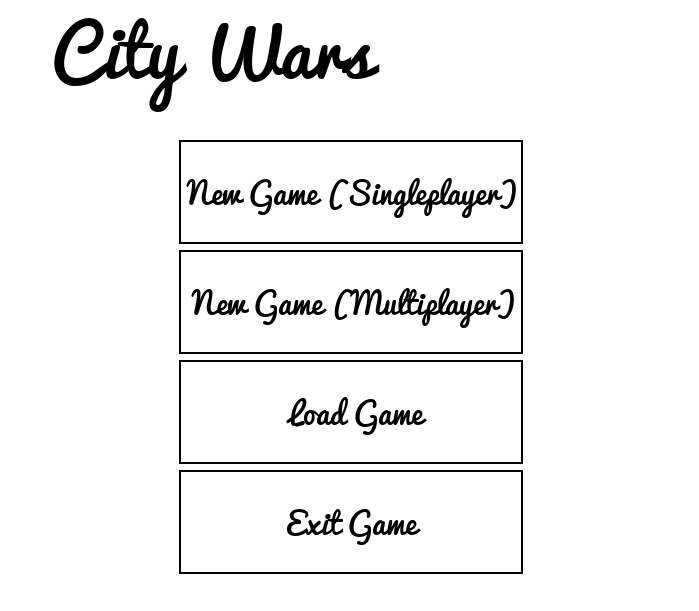
\includegraphics[width=\textwidth]{1.png}

V začetnem meniju igralec izbere ali želi igrati novo igro (zaenkrat je na voljo le način za enega igralca), ali pa želi naložiti že obstoječo igro, ki je lokalno shranjena.
Pred začetkom nove igre izbere svoje ime in število nasprotnikov (med 0 in 9). 

\subsection{Pogled mesta}

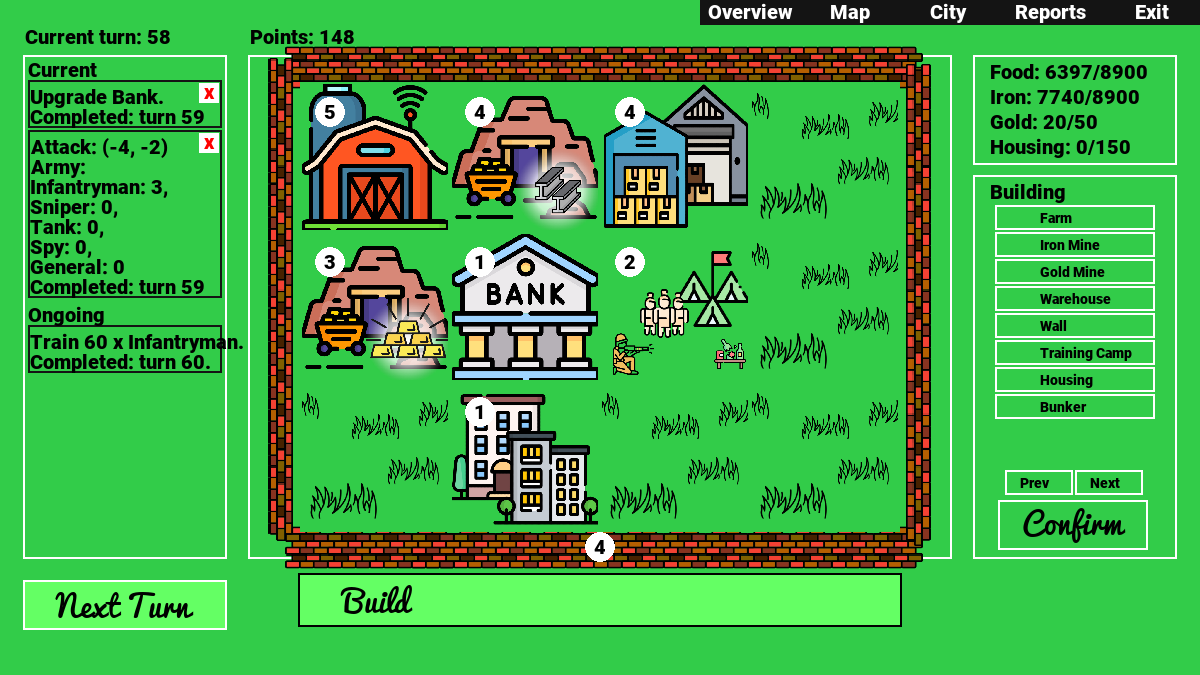
\includegraphics[width=\textwidth]{2.png}

V pogledu mesta igralec začenja vse akcije (z izjemo napadov). V tem pogledu so na voljo osnovne informacije o mestu.

\subsection{Pogled zemljevida}

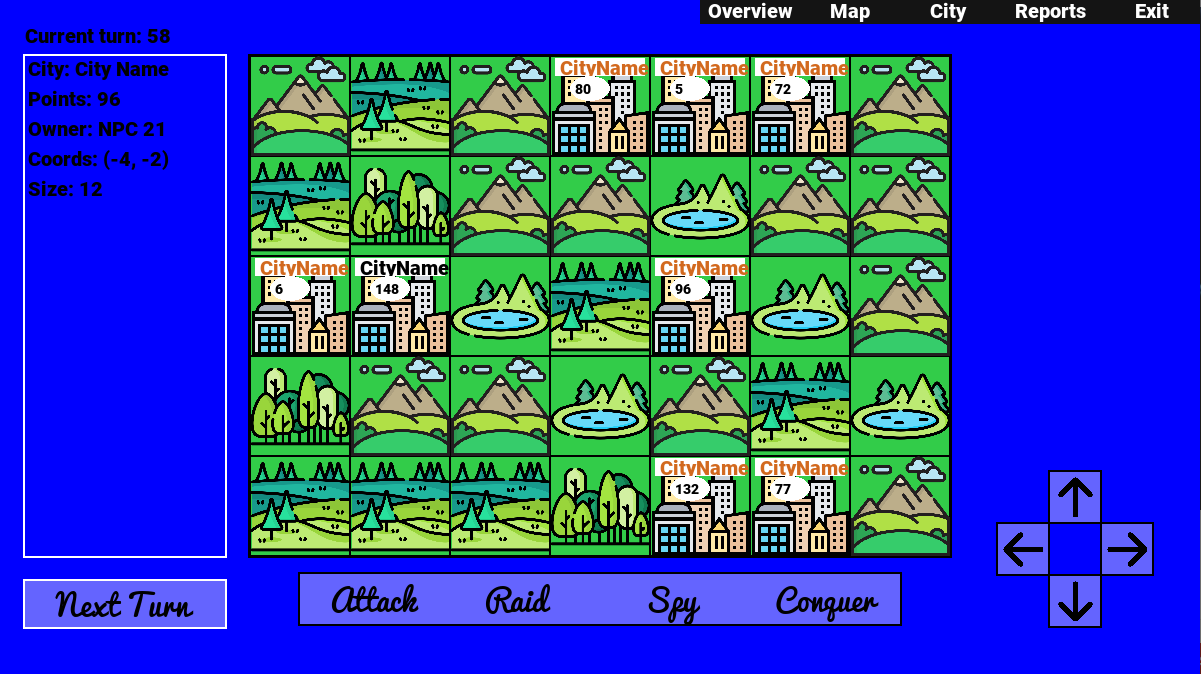
\includegraphics[width=\textwidth]{3.png}

V pogledu zemljevida igralec pošilja napadalne ukaze. Poleg tega so v tem pogledu na voljo informacije drugih mestih na svetu. Igralec lahko premika zemljevid s puščicami v desnem spodnjem kotu.


\end{document}